\documentclass{article}
\usepackage[T1]{fontenc}
\usepackage{lmodern}
\usepackage{graphicx}
\usepackage{amsmath,amssymb}
\usepackage[a4paper,margin=2cm]{geometry}
\usepackage[absolute,overlay]{textpos}
\setlength{\TPHorizModule}{1mm}
\setlength{\TPVertModule}{1mm}
\usepackage[indonesian]{babel}
\usepackage{hyperref}
\setlength{\emergencystretch}{2em}
% unit: Halaman 10

\begin{document}

% === Halaman 10 (llm) ===

\begin{itemize}
    \item Analogi pertukaran kunci Diffie-Hellman adalah seperti pertukaran cat antara dua orang (Alice dan Bob).
    \item Mula-mula Alice dan Bob menyepakati cat bersama yang warnanya tidak perlu rahasia (misalnya cat berwarna kuning)
    \item Masing-masing Alice dan Bob memiliki warna lain yang rahasia (dalam hal ini merah dan biru \textit{cyan})
    \item Alice dan Bob mencampurkan cat kuning dengan cat rahasia mereka masing-masing. Misalkan hasil pencampurannya adalah cat oranye dan cat biru terang
    \item Kemudian Alice dan Bob saling mempertukarkan cat hasil pencampuran tersebut (dikirim melalui transportasi umum).
    \item Selanjutnya, Alice dan Bob mencampurkan lagi cat rahasianya masing-masing dengan cat hasil pertukaran tersebut.
    \item Sekarang Alice dan Bob memiliki cat berwarna sama yang rahasia.
\end{itemize}

\vspace{10mm}

\begin{center}
    Rinaldi M/IL4020 Kriptografi
\end{center}

% deskripsi: Diagram ilustrasi analogi pertukaran kunci Diffie-Hellman menggunakan pencampuran warna cat antara Alice dan Bob.
% bbox normalisasi: [0.6300, 0.3600, 0.9800, 0.9300]
\begin{textblock*}{73.50mm}(132.30mm,106.92mm)
\noindent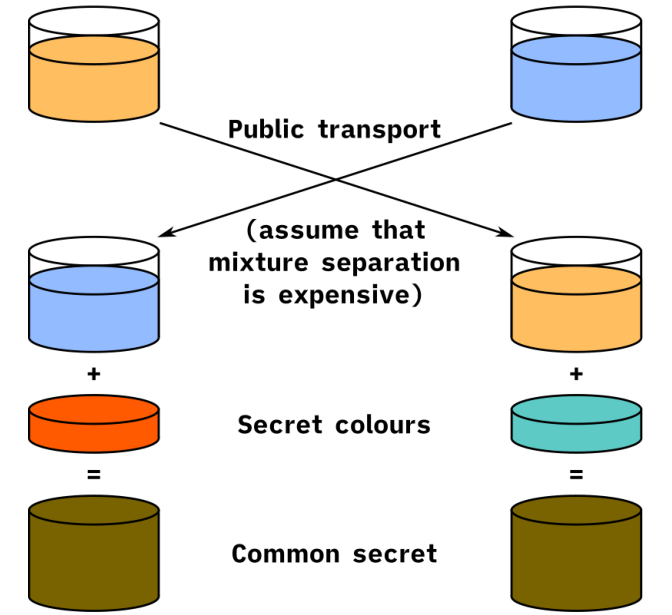
\includegraphics[width=73.50mm,height=169.29mm]{../../images/llm/page_010_img_01.png}%
\end{textblock*}

\end{document}
